\documentclass{article}

% if you need to pass options to natbib, use, e.g.:
% \PassOptionsToPackage{numbers, compress}{natbib}
% before loading nips_2016
%
% to avoid loading the natbib package, add option nonatbib:
% \usepackage[nonatbib]{nips_2016}

%\usepackage{nips_2016}

% to compile a camera-ready version, add the [final] option, e.g.:
 \usepackage[final]{nips_2016}

\usepackage[utf8]{inputenc} % allow utf-8 input
\usepackage[T1]{fontenc}    % use 8-bit T1 fonts
\usepackage{hyperref}       % hyperlinks
\usepackage{url}            % simple URL typesetting
\usepackage{booktabs}       % professional-quality tables
\usepackage{amsfonts}       % blackboard math symbols
\usepackage{nicefrac}       % compact symbols for 1/2, etc.
\usepackage{microtype}      % microtypography
\usepackage{graphicx}

\title{Proposal Template for Machine Learning Course}

% The \author macro works with any number of authors. There are two
% commands used to separate the names and addresses of multiple
% authors: \And and \AND.
%
% Using \And between authors leaves it to LaTeX to determine where to
% break the lines. Using \AND forces a line break at that point. So,
% if LaTeX puts 3 of 4 authors names on the first line, and the last
% on the second line, try using \AND instead of \And before the third
% author name.

\author{
  XXX\thanks{Use footnote for providing further
    information about author (webpage, alternative
    address)---\emph{not} for acknowledging funding agencies.} \\
  Department of Computer Science\\
  University of Iowa\\
  Iowa City, IA  52242 \\
  \texttt{xxx@uiowa.edu} \\
  %% examples of more authors
  %% \And
  %% Coauthor \\
  %% Affiliation \\
  %% Address \\
  %% \texttt{email} \\
  %% \AND
  %% Coauthor \\
  %% Affiliation \\
  %% Address \\
  %% \texttt{email} \\
  %% \And
  %% Coauthor \\
  %% Affiliation \\
  %% Address \\
  %% \texttt{email} \\
  %% \And
  %% Coauthor \\
  %% Affiliation \\
  %% Address \\
  %% \texttt{email} \\
}

\begin{document}
% \nipsfinalcopy is no longer used

\maketitle

\begin{abstract}
With the introduction of powerful telescopes such as the Hubble Space Telescope, vast quantities of high-fidelity imagery of remote galaxies have become available. Manual analysis of these images by experts has become infeasible, spawning citizen science projects such as Galaxy Zoo. However, the next generation of telescopes are expected to generate enormous volumes of data, going far beyond the capacity even of crowdsourced volunteers. In this study, we will extend the work done on automatic galaxy image classification in the Galaxy Zoo Kaggle challenge by developing a mapping between the various Galaxy Zoo "classification trees" and the popular Hubble Tuning Fork model. We will build a convolutional neural network to classify galaxies by leveraging the various crowdsourced Galaxy Zoo "gold standard" datasets. The model will be tested against expert-annotated classifications using third-party images.
\end{abstract}

\section{Introduction}
The size and scope of astronomy datasets has increased dramatically in recent years. The introduction of telescopes such as the Hubble Space Telescope (HST) and projects like the Sloan Digital Sky Survey (SDSS) have given astronomers access to imagery of millions of celestial objects. Traditional methods of data analysis, manually inspecting and classifying celestial objects, have become untenable in the face of this embarrassment of riches of data. 

Astronomers have successfully turned to citizen science projects such as Galaxy Zoo to leverage vast numbers of volunteers to help classify objects. The human visual system can, with little effort or training, provide image recognition capabilities that match or exceed the state of the art in computer image recognition. 

With the dawn of a new generation of telescopes, astronomy is threatened to be deluged in a sea of data. The GAIA spacecraft will produce a 3D map of over 1 billion astronomical objects. The Thirty Meter Telescope (TMT) and the 40-meter European Extremely Large Telecope (E-ELT) will view the visible universe at unprecedented depth. The Large Synoptic Survey Telescope (LSST) is estimated to generate 15 TB of data each night as it surveys the entire sky. Even these vast sums of data pale in comparision to the 1 TB/s output expected from the monsuvian Square Kilometer Array (SKA), which isn't limited to night time observing. Such enormous sums of data are beyond the ability of crowdsourcing to handle: they can only be handled by leveraging supercomputers, sophisticated algorithms, and machine learning.

The Galaxy Zoo Kaggle challenge was a competition in 2013 to produce a machine learning model that could replicate the classifications of citizen science volunteers on a dataset of 70000 galaxy images captured by HST. The top models performed very well in this challenge, but several questions remain. Can the galaxy classification scheme used by Galaxy Zoo be effectively mapped to astronomical classification schemes such as Hubble's Tuning Fork, or the more complex de Vaucouleurs system? Will machine learning models trained on the Galaxy Zoo dataset generalize well to other sources? 

To answer these questions, we will develop a mapping system between the various Galaxy Zoo “decision tree” classification schemes and the Hubble Tuning Fork scheme. We will develop a machine learning system to produce Tuning Fork classifications and train it on data from the Galaxy Zoo projects. We will then locate 3rd party datasets of expert-annotated galaxy images and test our system on these images. This project will investigate the generalizability of the Galaxy Zoo training data and the feasibility of mapping between the two galaxy classification schemes. 

\begin{figure}[h]
  \centering
	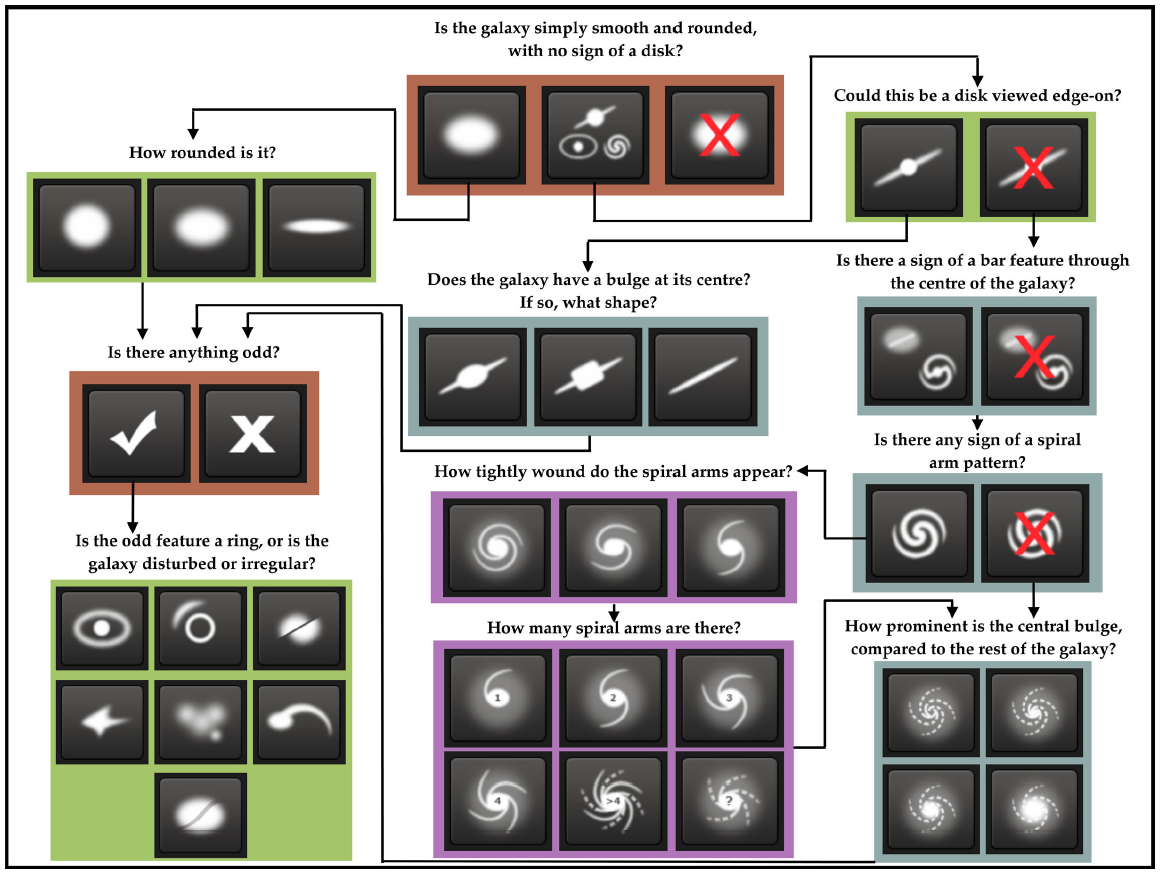
\includegraphics[width=100mm]{../img/GZ2_tree.png}
  \caption{The Galaxy Zoo 2 decision tree. Image from \cite{2013MNRAS.435.2835W}.}
\end{figure}

\section{Related Work}
\label{gen_inst}
In the astronomical community, the few automated galaxy classification systems have relied on more tradition methods, focusing on aggressive feature extraction algorithms making use of domain knowledge (such as WND-CHARM) to identify relationships among galaxies. These, however, have tended to focus on the more narrow classification of spirals and ellipticals, occasionally including edge-on spirals and irregular galaxies, and often work with much smaller datasets.

One example of the simple classification approach was done by \cite{2016ApJS..223...20K}, who, rather uniquely, made use of the ``super clean" galaxies from the Galaxy Zoo 1 catalog \citep{2008MNRAS.389.1179L} to classify 900 000 galaxies into spirals and ellipticals. They made use of an algorithm that extracted 2885 numerical descriptions from each image.

The Galaxy Zoo Kaggle challenge showed the power of convolutional neural networks (CNNs) when it comes to galaxy classification. Rather than relying on domain knowledge, the models had to learn to identify features on their own and were able to successfully reproduce the probabililty distributions of the citizen scientists. The winning model created 16 transformations for each image through the use of rotations and translations and trained the model on all 16 at once using convolutional layers and pooling.




\subsection{Figures}

All artwork must be neat, clean, and legible. Lines should be dark
enough for purposes of reproduction. The figure number and caption
always appear after the figure. Place one line space before the figure
caption and one line space after the figure. The figure caption should
be lower case (except for first word and proper nouns); figures are
numbered consecutively.

You may use color figures.  However, it is best for the figure
captions and the paper body to be legible if the paper is printed in
either black/white or in color.
\begin{figure}[h]
  \centering
  \fbox{\rule[-.5cm]{0cm}{4cm} \rule[-.5cm]{4cm}{0cm}}
  \caption{Sample figure caption.}
\end{figure}

\subsection{Tables}

All tables must be centered, neat, clean and legible.  The table
number and title always appear before the table.  See
Table~\ref{sample-table}.

Place one line space before the table title, one line space after the
table title, and one line space after the table. The table title must
be lower case (except for first word and proper nouns); tables are
numbered consecutively.

Note that publication-quality tables \emph{do not contain vertical
  rules.} We strongly suggest the use of the \verb+booktabs+ package,
which allows for typesetting high-quality, professional tables:
\begin{center}
  \url{https://www.ctan.org/pkg/booktabs}
\end{center}
This package was used to typeset Table~\ref{sample-table}.

\begin{table}[t]
  \caption{Sample table title}
  \label{sample-table}
  \centering
  \begin{tabular}{lll}
    \toprule
    \multicolumn{2}{c}{Part}                   \\
    \cmidrule{1-2}
    Name     & Description     & Size ($\mu$m) \\
    \midrule
    Dendrite & Input terminal  & $\sim$100     \\
    Axon     & Output terminal & $\sim$10      \\
    Soma     & Cell body       & up to $10^6$  \\
    \bottomrule
  \end{tabular}
\end{table}

\section{The Proposed Work}
Describe your proposed work in this section. 



\section{Plan}
Describe your plan for the project. What data you are going to use to evaluate your methods? What are the baselines that you want to compare? How will you develop your methods?   A timeline with important milestones is always perferred. 


\subsubsection*{Acknowledgments}

Use unnumbered third level headings for the acknowledgments. All
acknowledgments go at the end of the paper. Do not include
acknowledgments in the anonymized submission, only in the final paper.

\section*{References}

References follow the acknowledgments. Use unnumbered first-level
heading for the references. Any choice of citation style is acceptable
as long as you are consistent. It is permissible to reduce the font
size to \verb+small+ (9 point) when listing the references.

\begin{thebibliography}{9}
\bibitem[Dieleman et al.(2015)]{2015MNRAS.450.1441D} Dieleman, S., Willett, K.~W., \& Dambre, J.\ 2015, MNRAS, 450, 1441 
\bibitem[Kuminski \& Shamir(2016)]{2016ApJS..223...20K} Kuminski, E., \& Shamir, L.\ 2016, ApJS, 223, 20 
\bibitem[Lintott et al.(2008)]{2008MNRAS.389.1179L} Lintott, C.~J., Schawinski, K., Slosar, A., et al.\ 2008, MNRAS, 389, 1179
\bibitem[Szegedy et al.(2014)]{2014arXiv1409.4842S} Szegedy, C., Liu, W., Jia, Y., et al.\ 2014, arXiv:1409.4842 
\bibitem[Willett et al.(2013)]{2013MNRAS.435.2835W} Willett, K.~W., Lintott, C.~J., Bamford, S.~P., et al.\ 2013, MNRAS, 435, 2835  
\end{thebibliography}



\end{document}
